% Use class option [extendedabs] to prepare the 1-page extended abstract.
\documentclass[extendedabs]{bmvc2k}
\usepackage[colorlinks = true,
            linkcolor = blue,
            urlcolor  = blue,
            citecolor = blue,
            anchorcolor = blue]{hyperref}
\usepackage{kotex}
% for the fancy \koTeX logo
\usepackage{kotex-logo}

% Document starts here
\begin{document}


\title{VGGNet \& ResNet final-report}
\addauthor{
김태훈$^{1}$
}{}{1}

\addinstitution{
$^1$부산대학교 전기컴퓨터공학부.  
}
 
\maketitle
\noindent

\begin{figure}[t]
	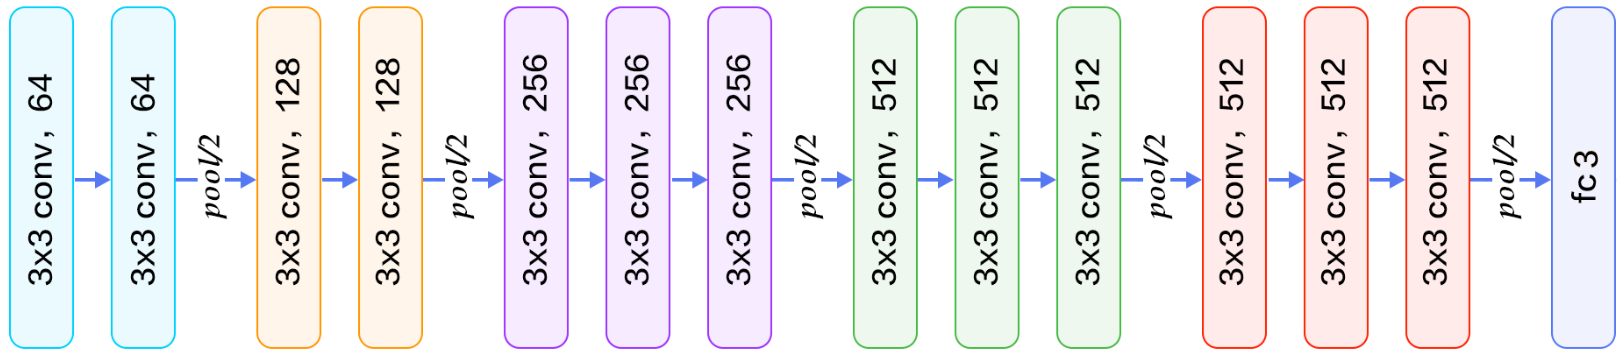
\includegraphics[width=\linewidth]{images/vggnet16.png}
	\caption{Configuration of VGG-16}
 \label{fig:VGGNet16}
	\vspace{-2mm}
\end{figure}

\section{Introduction}
VGGNet\cite{vggnet_paper} and ResNet\cite{resnet_paper} are CNN models that improve the performance of previous CNN models using increasing depth and residual learning framework respectively. VGGNet won the first place on the ImageNet Large-Scale Visualization Challenge(ILSVRC) 2014, and ResNet won the first place on the ILSVRC 2015. 

In this report, we use Pytorch to implement VGGNet and ResNet, and use CIFAR-10\cite{cifar10} datasets to train the CNN models for image classification, analyze and discuss the results.

\section{VGGNet}
\subsection{Dataset}
We use Images from the plane, car and bird categories in CIFAR-10 datasets. Each class consists of 6000 $32\times32$ color images. There are 5000 training images and 1000 test images in Each class. therefore there are 15000 training images and 3000 test images in total.
\subsection{Network architecture}
We use Type-D configuration in the paper\cite{vggnet_paper}, commonly known as VGG-16. Type-D configuration is shown on \ref{fig:VGGNet16}.

Since we use $32\times32$ CIFAR-10 images, the last 3 FC(fully connected) layer are different from the VGGNet in the paper\cite{vggnet_paper} that using Imagenet dataset resized into $224\times224$. $32x32$ images change to $1\times1\times512$ feature maps after VGG16 convolutional layers. furthermore, We use 3 categories images. Therefore, Our VGG16 model have 1 FC layer that classify input to 3 categories\ref{tab:vggnetwithcifar10}

All hidden layers are equipped with the ReLU\cite{alexnet}, and batch normal-ization\cite{batchnorm} is incorporated after every convolution, which helps in stabilizing and accelerating the training process, and which is not used in the paper\cite{vggnet_paper}. Thus, after each convolution, batch normalization and ReLU are applied in order. Also, there are no dropout layers for simplicity. The number of parameters is about 14.7M.

\subsection{Loss function} \label{lossfunction}
We use Cross-entropy loss between outputs and targets as loss function. Since nn.CrossEntropyLoss function takes logits before softmax as outputs and scaler-index as targets, We don't apply a softmax function after the output layer. 

\begin{table}[]
\centering
\begin{tabular}{|lll|}
\hline
\multicolumn{3}{|l|}{VGG-16 with (mini-) CIFAR-10 config}                           \\ \hline
\multicolumn{1}{|l|}{layer name} & \multicolumn{1}{l|}{output size} &               \\ \hline
\multicolumn{1}{|l|}{conv1\_x}   & \multicolumn{1}{l|}{32x32x64}    & (3x3, 64) x2  \\ \hline
\multicolumn{1}{|l|}{pool1}      & \multicolumn{1}{l|}{16x16x64}    & maxpool       \\ \hline
\multicolumn{1}{|l|}{conv2\_x}   & \multicolumn{1}{l|}{16x16x128}   & (3x3, 128) x2 \\ \hline
\multicolumn{1}{|l|}{pool2}      & \multicolumn{1}{l|}{8x8x128}     & maxpool       \\ \hline
\multicolumn{1}{|l|}{conv3\_x}   & \multicolumn{1}{l|}{8x8x256}     & (3x3, 256) x3 \\ \hline
\multicolumn{1}{|l|}{pool3}      & \multicolumn{1}{l|}{4x4x256}     & maxpool       \\ \hline
\multicolumn{1}{|l|}{conv4\_x}   & \multicolumn{1}{l|}{4x4x512}     & (3x3, 512) x3 \\ \hline
\multicolumn{1}{|l|}{pool4}      & \multicolumn{1}{l|}{2x2x512}     & maxpool       \\ \hline
\multicolumn{1}{|l|}{conv5\_x}   & \multicolumn{1}{l|}{2x2x512}     & (3x3, 512) x3 \\ \hline
\multicolumn{1}{|l|}{pool5}      & \multicolumn{1}{l|}{1x1x512}     & maxpool       \\ \hline
\multicolumn{1}{|l|}{fc-3}        & \multicolumn{1}{l|}{3}         & (512, 3)    \\ \hline

\end{tabular}

\caption{Configuration of VGG-16 with CIFAR-10 config}
\label{tab:vggnetwithcifar10}
\end{table}


\subsection{Training} \label{trainingsection}
The training is carried out by optimising the multiple logistic regression, using mini-match stochastic gradient descent optimizer with momentum. The optimizing method is back-propagation\cite{backpropagation}.
The batch size was set to 128, momentum to 0.9, learning rate to $10^{-2}$, and weight-decay to  $5\times10^{-4}$.Additionally, we trained the models for 20 epochs without learning rate scheduling. For simplicity, weight was initialized with default Pytorch weight initialization method.

The training images size was fixed to 32x32. The training images was preprocessed with random cropping to 32x32(The images was padded 4 for all direction before cropped), random horizontal fliping, changing images array to Pytorch tensors(which changes $Height\times Width\times Channel$ to $Channel\times Height\times Width$ and scale RGB values to 0 to 1), and normalizing pixels with mean and standard of RGB values of training images.

\subsection{Testing}
We tested the models for every epochs with test images. Test images was preprocessed with changing images array to Pytorch tensors and normalizing pixels with mean and standard of RGB values of training images. Random cropping and horizontal fliping was not applied to the test images because of consistency of testing. Testing method is classification accuracy(i.e., the precentage of correct prediction.
\subsection{Implementation Details}
\subsubsection{Configuration array}
The Configuration array(declared a 'cfg' on code) defines the architecture configuration of the VGG16 model. It specified the number of output channels for each convolutional layer and the placement of max pooling layers('MP').
\subsubsection{Model Class}
The Model Class, declared a 'VGG' on code, inherits from nn.Module. Attributes of the class defines the convolutional layers and fully connected layers. The convolutional layers declared a attribute 'VGG16': The make-layers method constructs the convolutional part of the network based on the cfg configuration. For each integer value in cfg, nn.Conv2d with output channels is added, followed by nn.BatchNorm2d and nn.ReLU. When a 'MP' is encountered, nn.MaxPool2d is added.

Fully Connected Layers declared a attribute 'classifier': there is one FC layer with 3 channels for classification tasks.

Forward Pass method consists of 3 steps: Convolutional Processing, Flattening, and Classification. Convolutional processing is that Input data x is passed through the convolutional layers. Flattening is that the output feature maps are reshaped into a 1D tensor using out.view(out.size(0), -1) for the fully connected layers. Classification is that the flattened tensor is passed the classifier to obtain the final logit values.

\subsection{Results}
After the final epochs, Training loss and Testing accuracy was about 0.0004 and 91.2 each\ref{tab:testresults}. Training loss and testing accuracy on every epoch show on fig\ref{fig:VGGNet16lossacc}

\section{ResNet}
\subsection{Dataset}
We use the dataset that used for VGGNet.
\subsection{Network Architecture}
We use 50-layer ResNet(i.e., ResNet50) with bottleneck blocks. The configuration of ResNet50 is different from the paper\cite{resnet_paper}, first is the initial convolutional layer changed from $7\times7,64, stride=2$ to $3\times3, 64, stride=1$, and second is the initial max-pooling layer is removed because the size of CIFAR-10\cite{cifar10} images is too small. 

The configuration of ResNet50 for CIFAR-10\cite{cifar10} is \ref{fig:resnetfig}, and the residual connection is \ref{fig:resconnection}. All hidden layers(except the convolution layer for expanding channels) are equipped with the ReLU\cite{alexnet}, and batch normal-ization\cite{batchnorm} is incorporated after every convolution. Strided convolution for down-sampling instead of max-pooling layer. if Once down-sampled, a $1\times1$ convolution with stride 2 is applied to residual input for matching dimension of input and output. if down-sampling is not applied but the number of channels of input and output are different(i.e., the first block of cfg[0] blocks in \ref{fig:resnetfig}), convolution with stride 1 is applied to residual input for expanding channels of input. Also, there are no dropout for simplicity. The number of parameters is about 23.5M.

\subsection{Loss Function}
The loss function is same with VGGNet above\ref{lossfunction}. In other words, Cross-entropy loss between outputs and ground-truths.

\subsection{training}
The training method is same with VGGNet above\ref{trainingsection}, except the number of epochs is 15.

\subsection{implementation Details}
\subsubsection{configuration array}
The configuration array('cfg' variable in code) defines the number of residual blocks in each of the four main residual net layers of the ResNet50. [3,4,6,3] indicates that Layer1-Layer4 has 3, 4, 6, 3 residual blocks each.
\subsubsection{ResNet block class}
ResNet block class defines a single residual block. The arguments of initialization of resnet block class is 'in-c', 'intra-c','out-c', 'down-sample', 'expand'. Each block consists of three convolution layers:

\textbf{First Convolution} conv1 consists of $1\times1$ convolution, Batch Normalization, and ReLU. $1\times1$ convolution reduces number of channels from 'in-c' to 'intra-c'. if 'down-sample' arguments is true, then stride of convolution is 2 for downsampling.

\textbf{Second Convolution} conv2 consists of $3\times3$ convolution, and others are same with conv1. $3\times3$ convolution layer maintain the number of channels(in-tra-c), and padding='same' to preserve spatial dimensions.

\textbf{Third Convolution} conv3 consists of $1\times1$ convolution, and Batch Normalization. $1\times1$ convolution expands the number of channels from intra-c to out-c.

If down-sample or expand attribute is true, the input undergoes a $1\times1$ convolution to match the dimensions of the output from the convolution layers. if down-sample is true, the stride of $1\times1$ convolution is 2(if not, then stride is 1). The output of the convolution layers is added to the input, and a ReLU activation is applied.

this residual connection enables the network to learn identity mapping and thus allowing the construction of deeper networks without vanishing or exploding gradient.



\begin{table}[]
\centering
\begin{tabular}{|ccc|}
\hline
\multicolumn{3}{|c|}{VGG-16 with (mini-) CIFAR-10 config}                                \\ \hline
\multicolumn{1}{|c|}{layer name} & \multicolumn{1}{c|}{output size} &                    \\ \hline
\multicolumn{1}{|c|}{conv1\_x}   & \multicolumn{1}{c|}{32x32x64}    & (3x3, 64) stride 1 \\ \hline
\multicolumn{1}{|c|}{conv2\_x}   & \multicolumn{1}{c|}{32x32x256}   & $\left[\begin{array}{cc}1\times1, 64  \\3\times3, 64  \\1\times1, 256 \\\end{array}\right] \times 3$           \\ \hline
\multicolumn{1}{|c|}{conv3\_x}   & \multicolumn{1}{c|}{16x16x512}   & $\left[\begin{array}{cc}1\times1, 128  \\3\times3, 128  \\1\times1, 512 \\\end{array}\right] \times 4$            \\ \hline
\multicolumn{1}{|c|}{conv4\_x}   & \multicolumn{1}{c|}{8x8x1024}    & $\left[\begin{array}{cc}1\times1, 256  \\3\times3, 256  \\1\times1, 1024 \\\end{array}\right] \times 6$             \\ \hline
\multicolumn{1}{|c|}{conv5\_x}   & \multicolumn{1}{c|}{4x4x2048}    & $\left[\begin{array}{cc}1\times1, 512  \\3\times3, 512  \\1\times1, 2048 \\\end{array}\right] \times 3$            \\ \hline
\multicolumn{1}{|c|}{avgpool}    & \multicolumn{1}{c|}{2048}        &             \\ \hline
\multicolumn{1}{|c|}{fc1}        & \multicolumn{1}{c|}{3}           &             \\ \hline
\end{tabular}
\caption{Configuration of ResNet50 with CIFAR-10 config}
\label{tab:resnetconfig}
\end{table}

\begin{table}[]
\centering
\begin{tabular}{|l|l|l|}
\hline
                  & VGG16  & ResNet50 \\ \hline
Train Loss         & 0.0004  & 0.0586    \\ \hline
Test Accuracy(\%) & 91.2 & 85.8333   \\ \hline
\end{tabular}
\caption{Train loss and test accuracy of VGG16 and ResNet50. the values was rounded off to the the fourth decimal place.}
\label{tab:testresults}
\end{table}

\begin{figure}[t]
	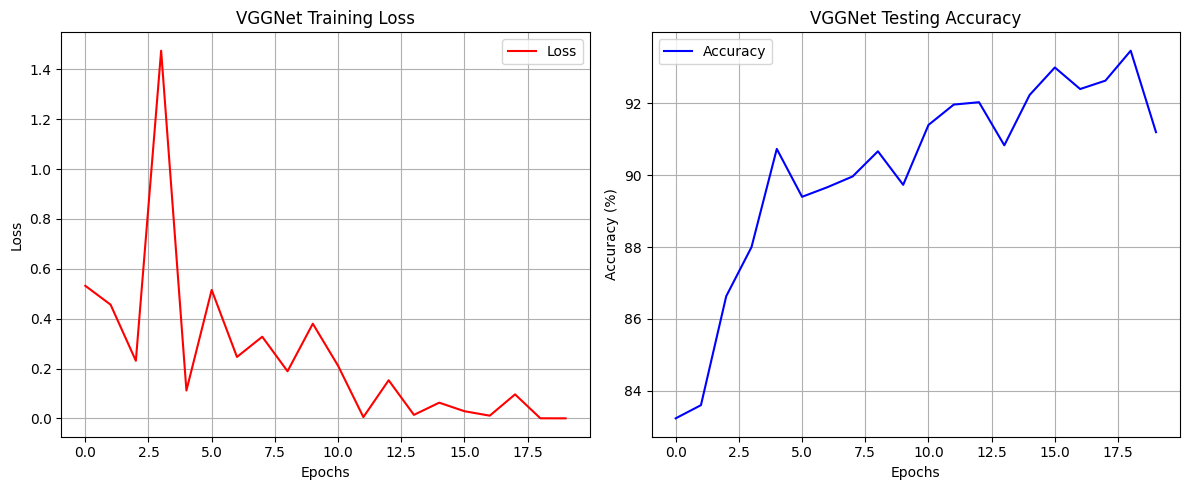
\includegraphics[width=\linewidth]{images/vggnetlossacc.png}
	\caption{Training loss(left) and Testing accuracy(right) on CIFAR-10\cite{cifar10} with VGG16 networks.}
 \label{fig:VGGNet16lossacc}
	\vspace{-2mm}
\end{figure}

\begin{figure}[t]
	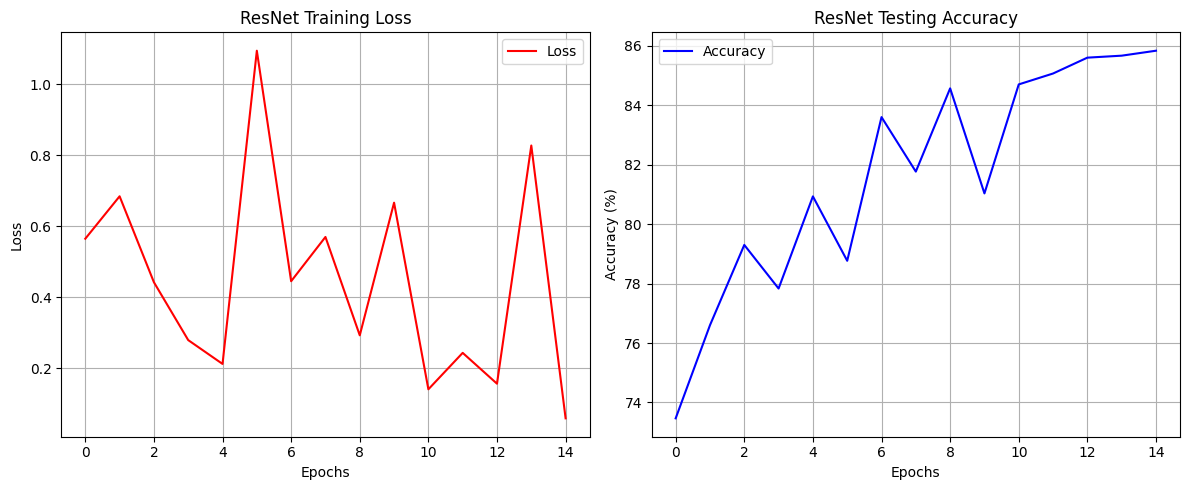
\includegraphics[width=\linewidth]{images/resnetlossacc.png}
	\caption{Training loss(left) and Testing accuracy(right) on CIFAR-10 with ResNet50 networks.}
 \label{fig:ResNetlossacc}
	\vspace{-2mm}
\end{figure}

\begin{figure}[htb!]
	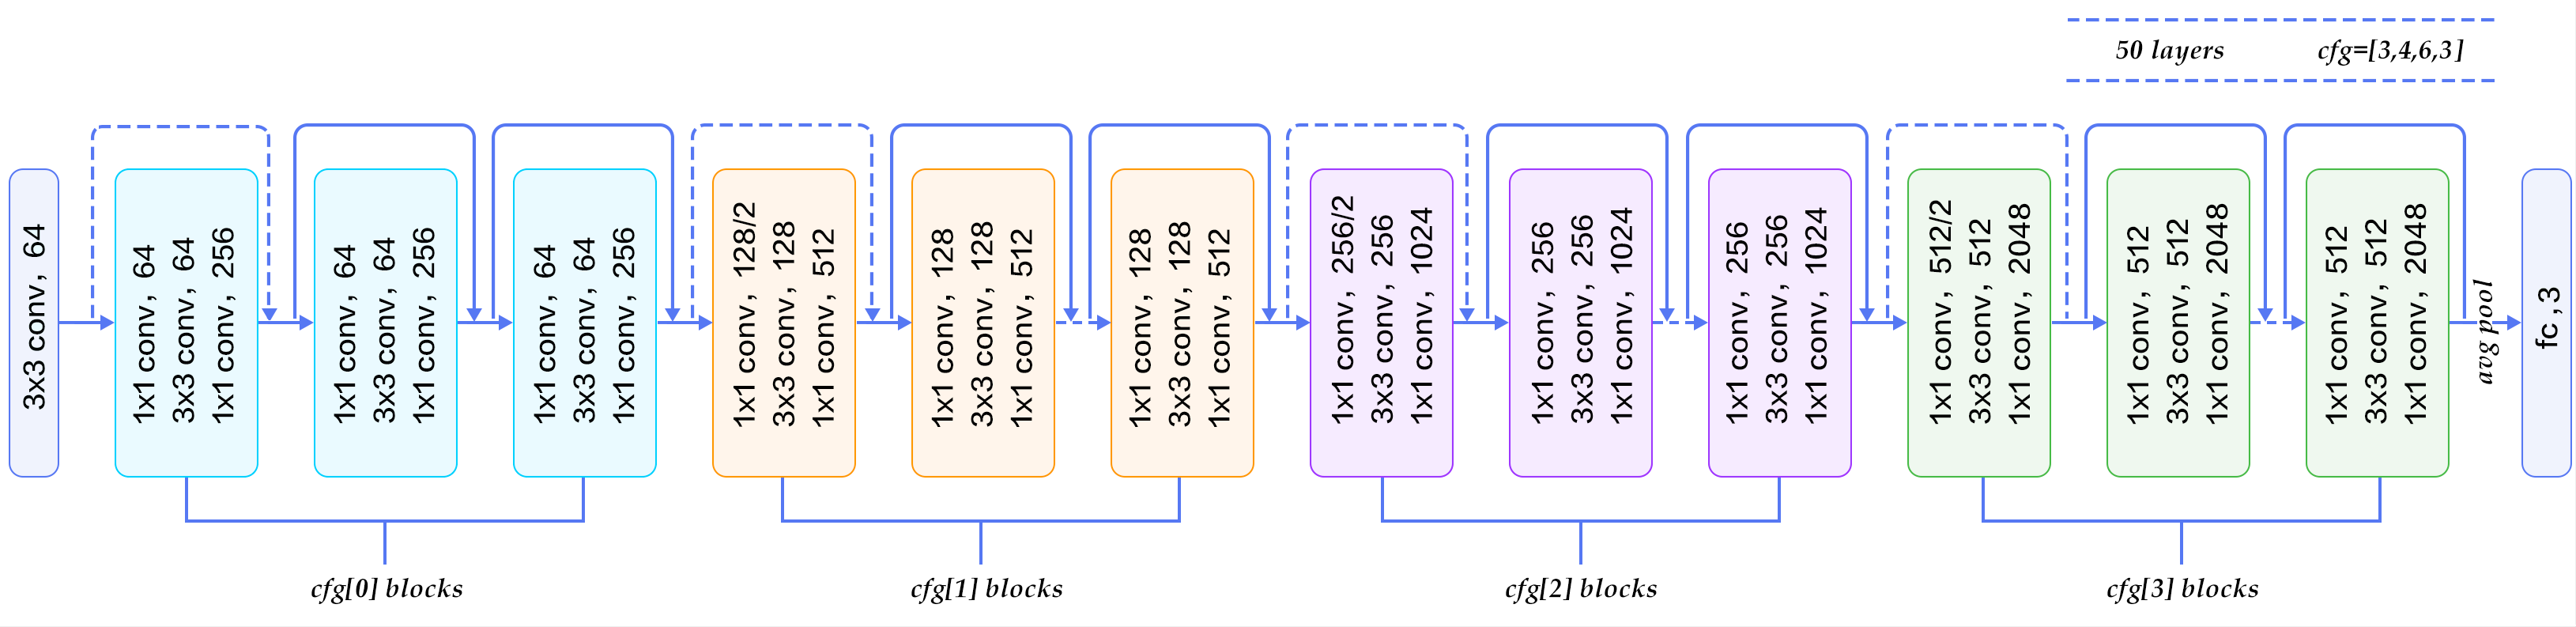
\includegraphics[width=\linewidth]{images/resnet_fig.png}
	\caption{Architecture of resnet50 for CIFAR-10\cite{cifar10}. solid line means the normal residual connection(left part of \ref{fig:resconnection}), and dotted line means the residual connection with channel expanding(right part of \ref{fig:resconnection})}
 \label{fig:resnetfig}
	\vspace{-2mm}
\end{figure}

\begin{figure}[htb!]
	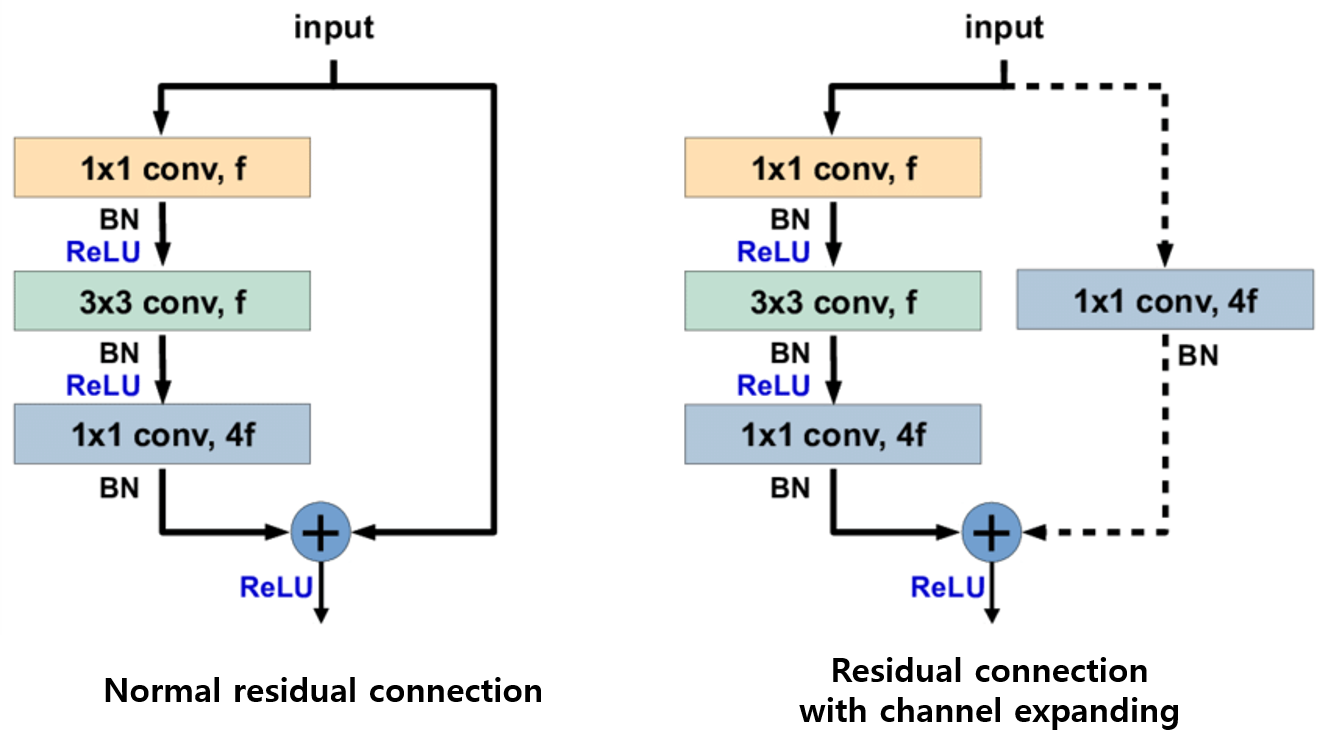
\includegraphics[width=\linewidth]{images/res_connection.png}
	\caption{Normal residual connection(left) and Residual connection with channel expanding(right). If input dimensions and output dimensions are different, input channel expanding should be applied before adding to output}
 \label{fig:resconnection}
	\vspace{-2mm}
\end{figure}

\subsubsection{ResNet Model Class}
The ResNet class defines the entire ResNet50 architecture. The class consists of initial block, residual layers, adaptive average pooling and classifier. initial block consists of $3\times3$ convolution that number of output channels is 64, Batch Normalization and ReLU activation. Residual layers are like \ref{fig:resnetfig}\ref{tab:resnetconfig}

The forward of this model has 4 part: Initial convolutional processing, passing residual layers, global average pooling, flattening, and classification.

Initial convolutional processing is that the input tensor passes through the initial block. passing residual layers is that the output from initial block sequentially passes through first to fourth residual block. global average pooling is that the output from the last residual layer undergoes adaptive average pooling,which changes feature map dimension from $Height\times Width \times Channels$ to $1\times1\times Channel$. Finally, flattening and classification is that changes feature map to 1D tensor, and passed through classifier, which consists of a linear layers that maps the features to logit values.

\subsection{Results}
After the final epochs, Training loss and Testing accuracy was about 0.0586 and 85.8333 each\ref{tab:testresults}. Training loss and testing accuracy on every epoch show on fig\ref{fig:ResNetlossacc}

\section{Discussion}
For both models, The training loss graph is fluctuating, which might suggest issues with the large learning rate. Applying the Adam optimizer\cite{adamopt} or setting learning rate to be smaller may resolve the issue. The test accuracy of both models are higher than 85\%, which shows that deeper layer improve the performance. Deeper layers have ability to represent complex function, and hierarchical learning. VGG16 is better than ResNet50 in training loss and testing accuracy. That may be because ResNet has more parameters and deeper layers than VGGNet, making 15,000 training data insufficient to train all of its parameters. If there are more training data(and more categories), ResNet may be better than VGGNet because ResNet50 is better than VGG16 in the ResNet paper\cite{resnet_paper}, which trained the models with ImageNet. Also, dropout layers may help improving test accuracy with overfitting prevention.
\section{Conclusion}
In this lab, We implemented The VGGNet16 and ResNet50 using Pytorch, training and testing the models with first 3-categories CIFAR-10 images. Additionally, we compared the performance of VGGNet and ResNet on the CIFAR-10 image classification task. Our experiments showed that the test accuracy of both models greater than 85\%, and VGG16 achieved a lower training loss with higher testing accuracy.

This result suggests that deeper layers improve the performance, ResNet50 need more data because of it has more parameters, and VGGNet may be more suitable for less complex dataset like CIFAR-10. However, it is useful to consider ResNet's advantages like residual connections. ResNet may become more powerful on larger image datasets. Therefore, It is important that selecting appropriate architectures based on the characteristic like size of the datasets.

\newpage
\bibliography{egbib}

\end{document}
